\begin{ujnbody}
    \section{基础功能测试}
    \subsection{文字与段落}
    这是文字\cite{zh-book-8},这是参考文献的交叉引用\cite{shannon1948mathematical}。

    这是段落。这是段落。这是段落。这是段落。这是段落。这是段落。这是段落。这是段落。这是段落。这是段落。这是段落。这是段落。这是段落。这是段落。这是段落。这是段落。这是段落。这是段落。
    \subsubsection{文字与段落}
    这是文字,这是参考文献的交叉引用\cite{nash1996non}。

    这是段落\cite{zh-book-9},这是参考文献的交叉引用\cite{turing2009computing}。这是段落。这是段落。这是段落。这是段落。这是段落。这是段落。这是段落。这是段落。这是段落。这是段落。这是段落。这是段落。这是段落。这是段落。这是段落。这是段落。这是段落。
    \subsection{图表}

    \subsubsection{图片}

    \begin{figure}[htbp]
        \centering
        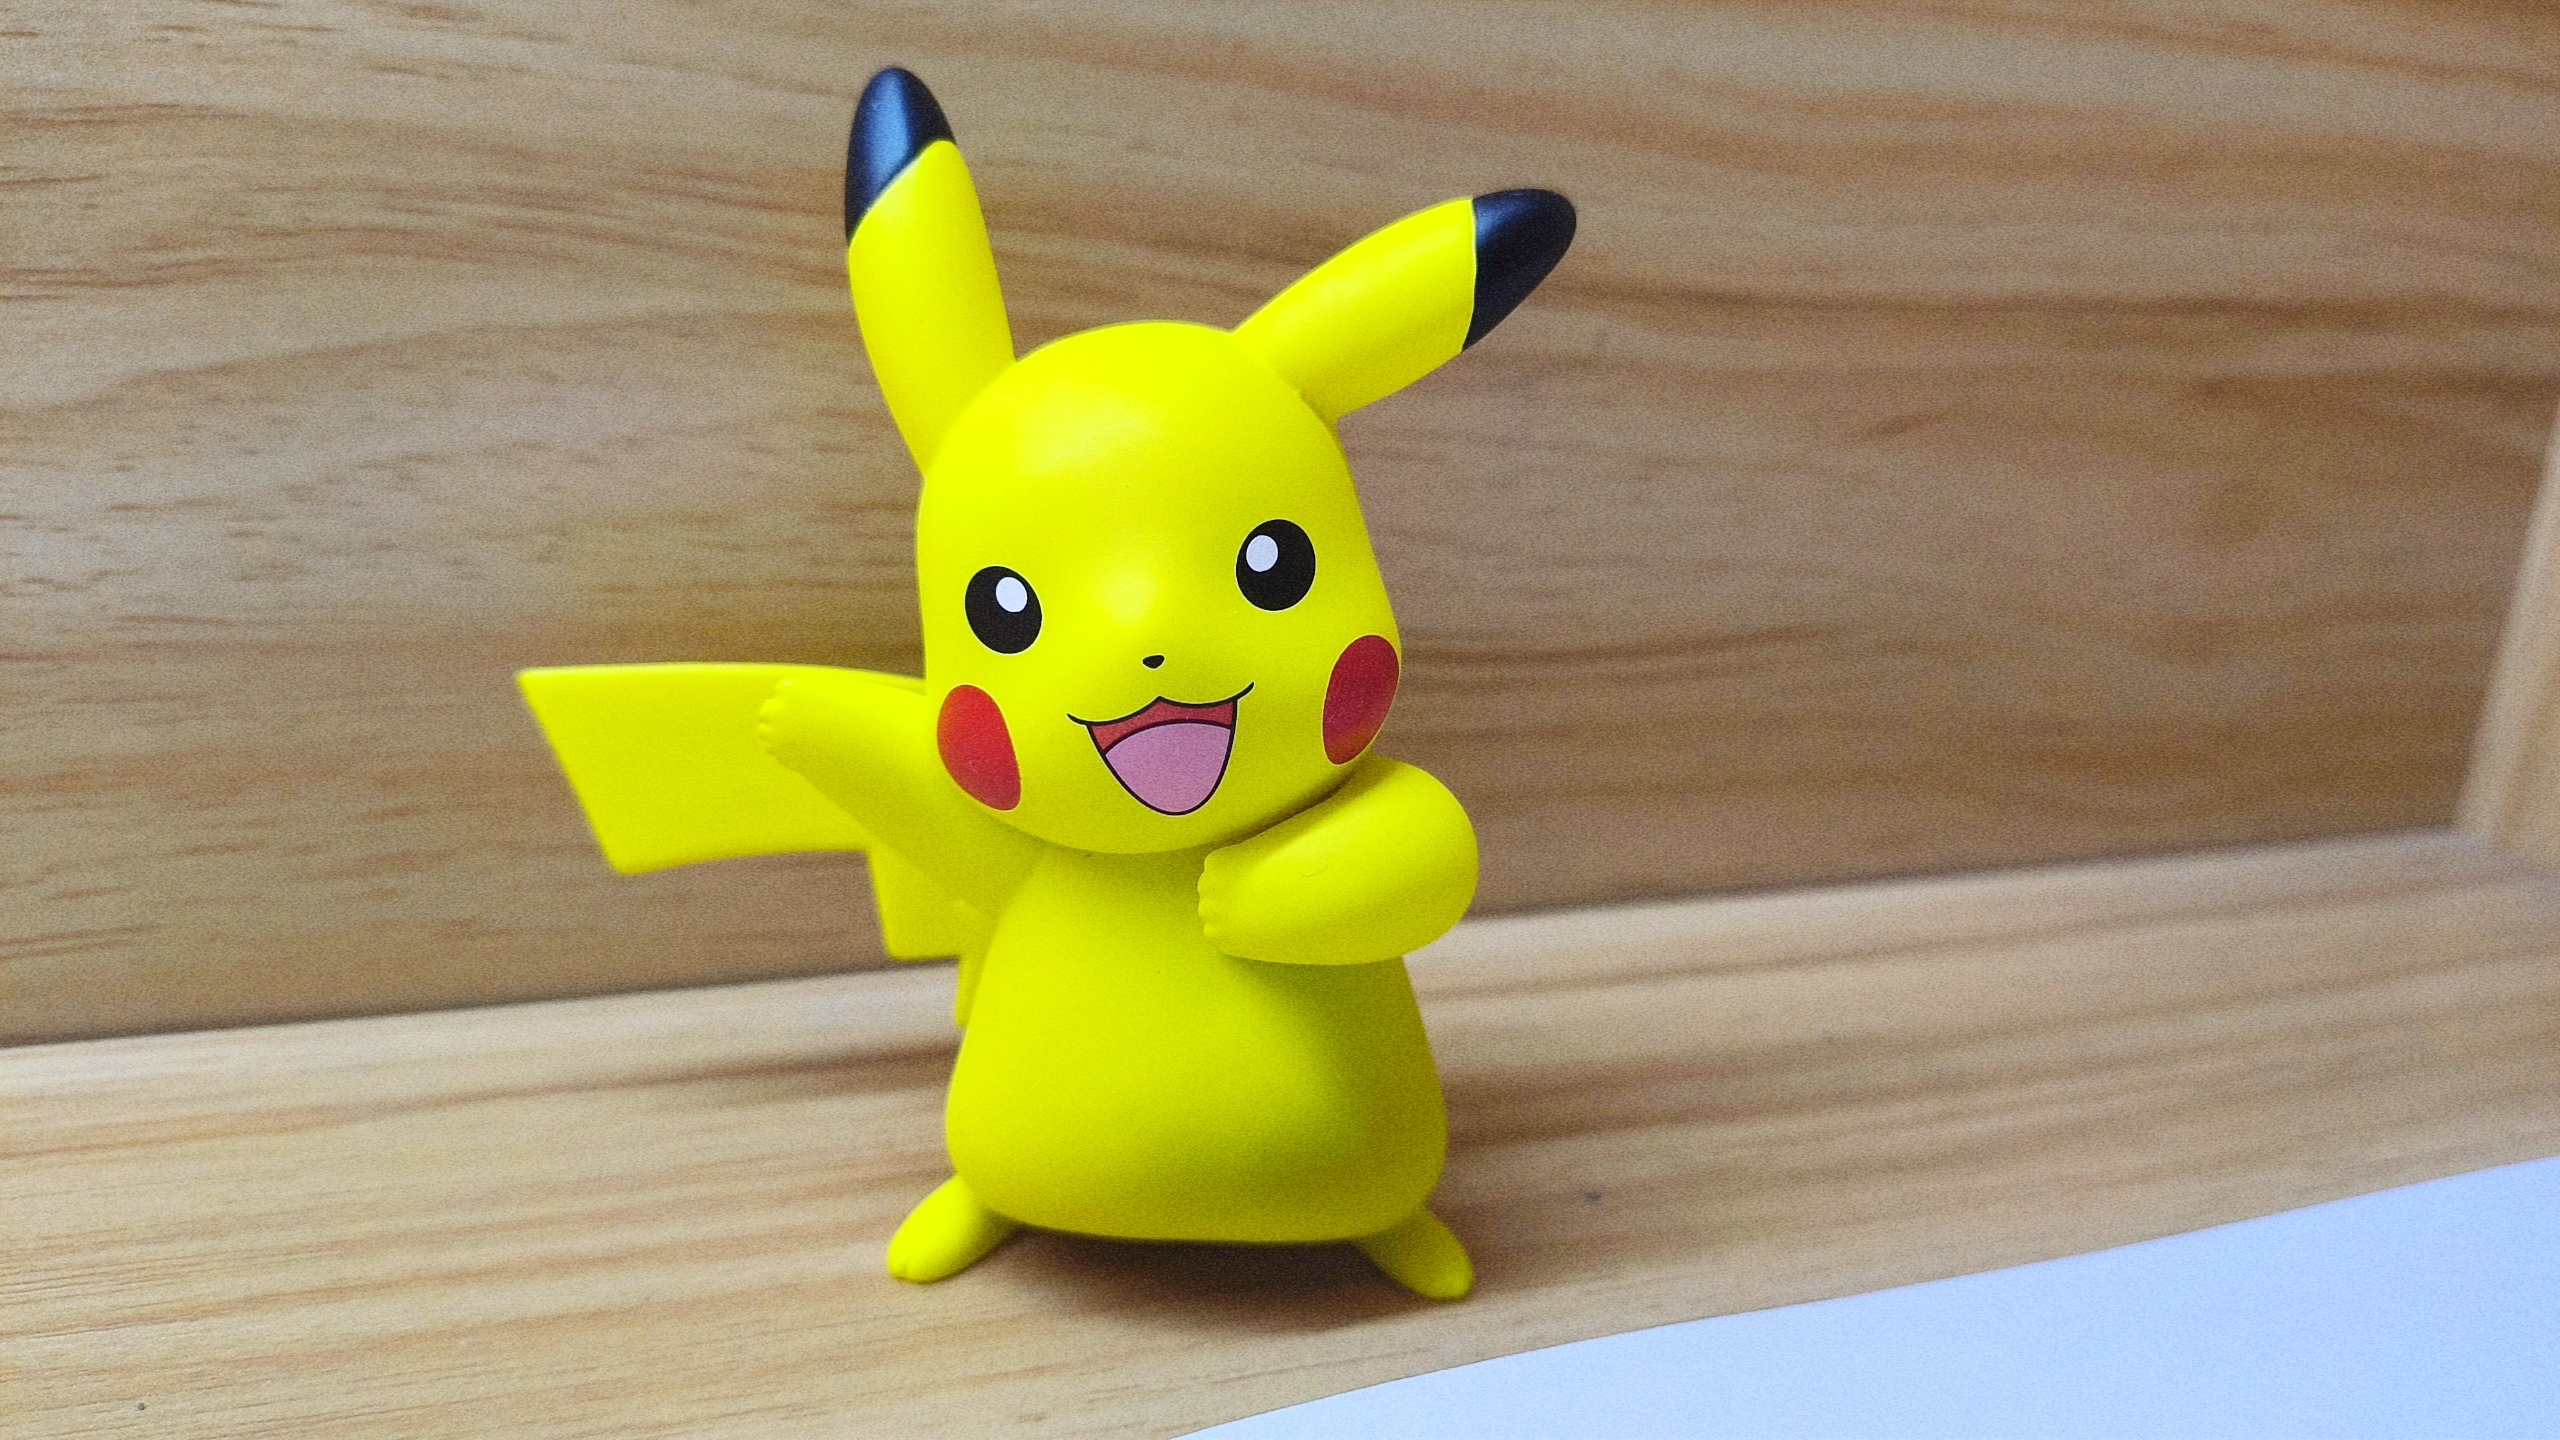
\includegraphics[scale=0.1, ]{figures/pikachu.jpg}
        \caption{这是图表}
        %\label{fig:1}
    \end{figure}

    \subsubsection{表格}

    \begin{table}[!htbp]
        \centering
        \begin{tabular}{cccccc}
            \toprule
            序号 & 姓名 & 性别 & 年龄 & 身高/cm & 体重/kg \\
            \midrule
            1 & 张三 & M & 16 & 163 & 50 \\
            2 & 王红 & F & 15 & 159 & 47 \\
            3 & 李二 & M & 17 & 165 & 52 \\
            \bottomrule
        \end{tabular}
        \caption{这是表格}
    \end{table}

    \section{基础功能测试}
    \subsection{文字与段落}
    这是文字。

    这是段落。这是段落。这是段落。这是段落。这是段落。这是段落。这是段落。这是段落。这是段落。这是段落。这是段落。这是段落。这是段落。这是段落。这是段落。这是段落。这是段落。这是段落。
    \subsubsection{文字与段落}
    这是文字。

    这是段落。这是段落。这是段落。这是段落。这是段落。这是段落。这是段落。这是段落。这是段落。这是段落。这是段落。这是段落。这是段落。这是段落。这是段落。这是段落。这是段落。这是段落。
    \subsection{图表}

    \subsubsection{图片}

    \begin{figure}[htbp]
        \centering
        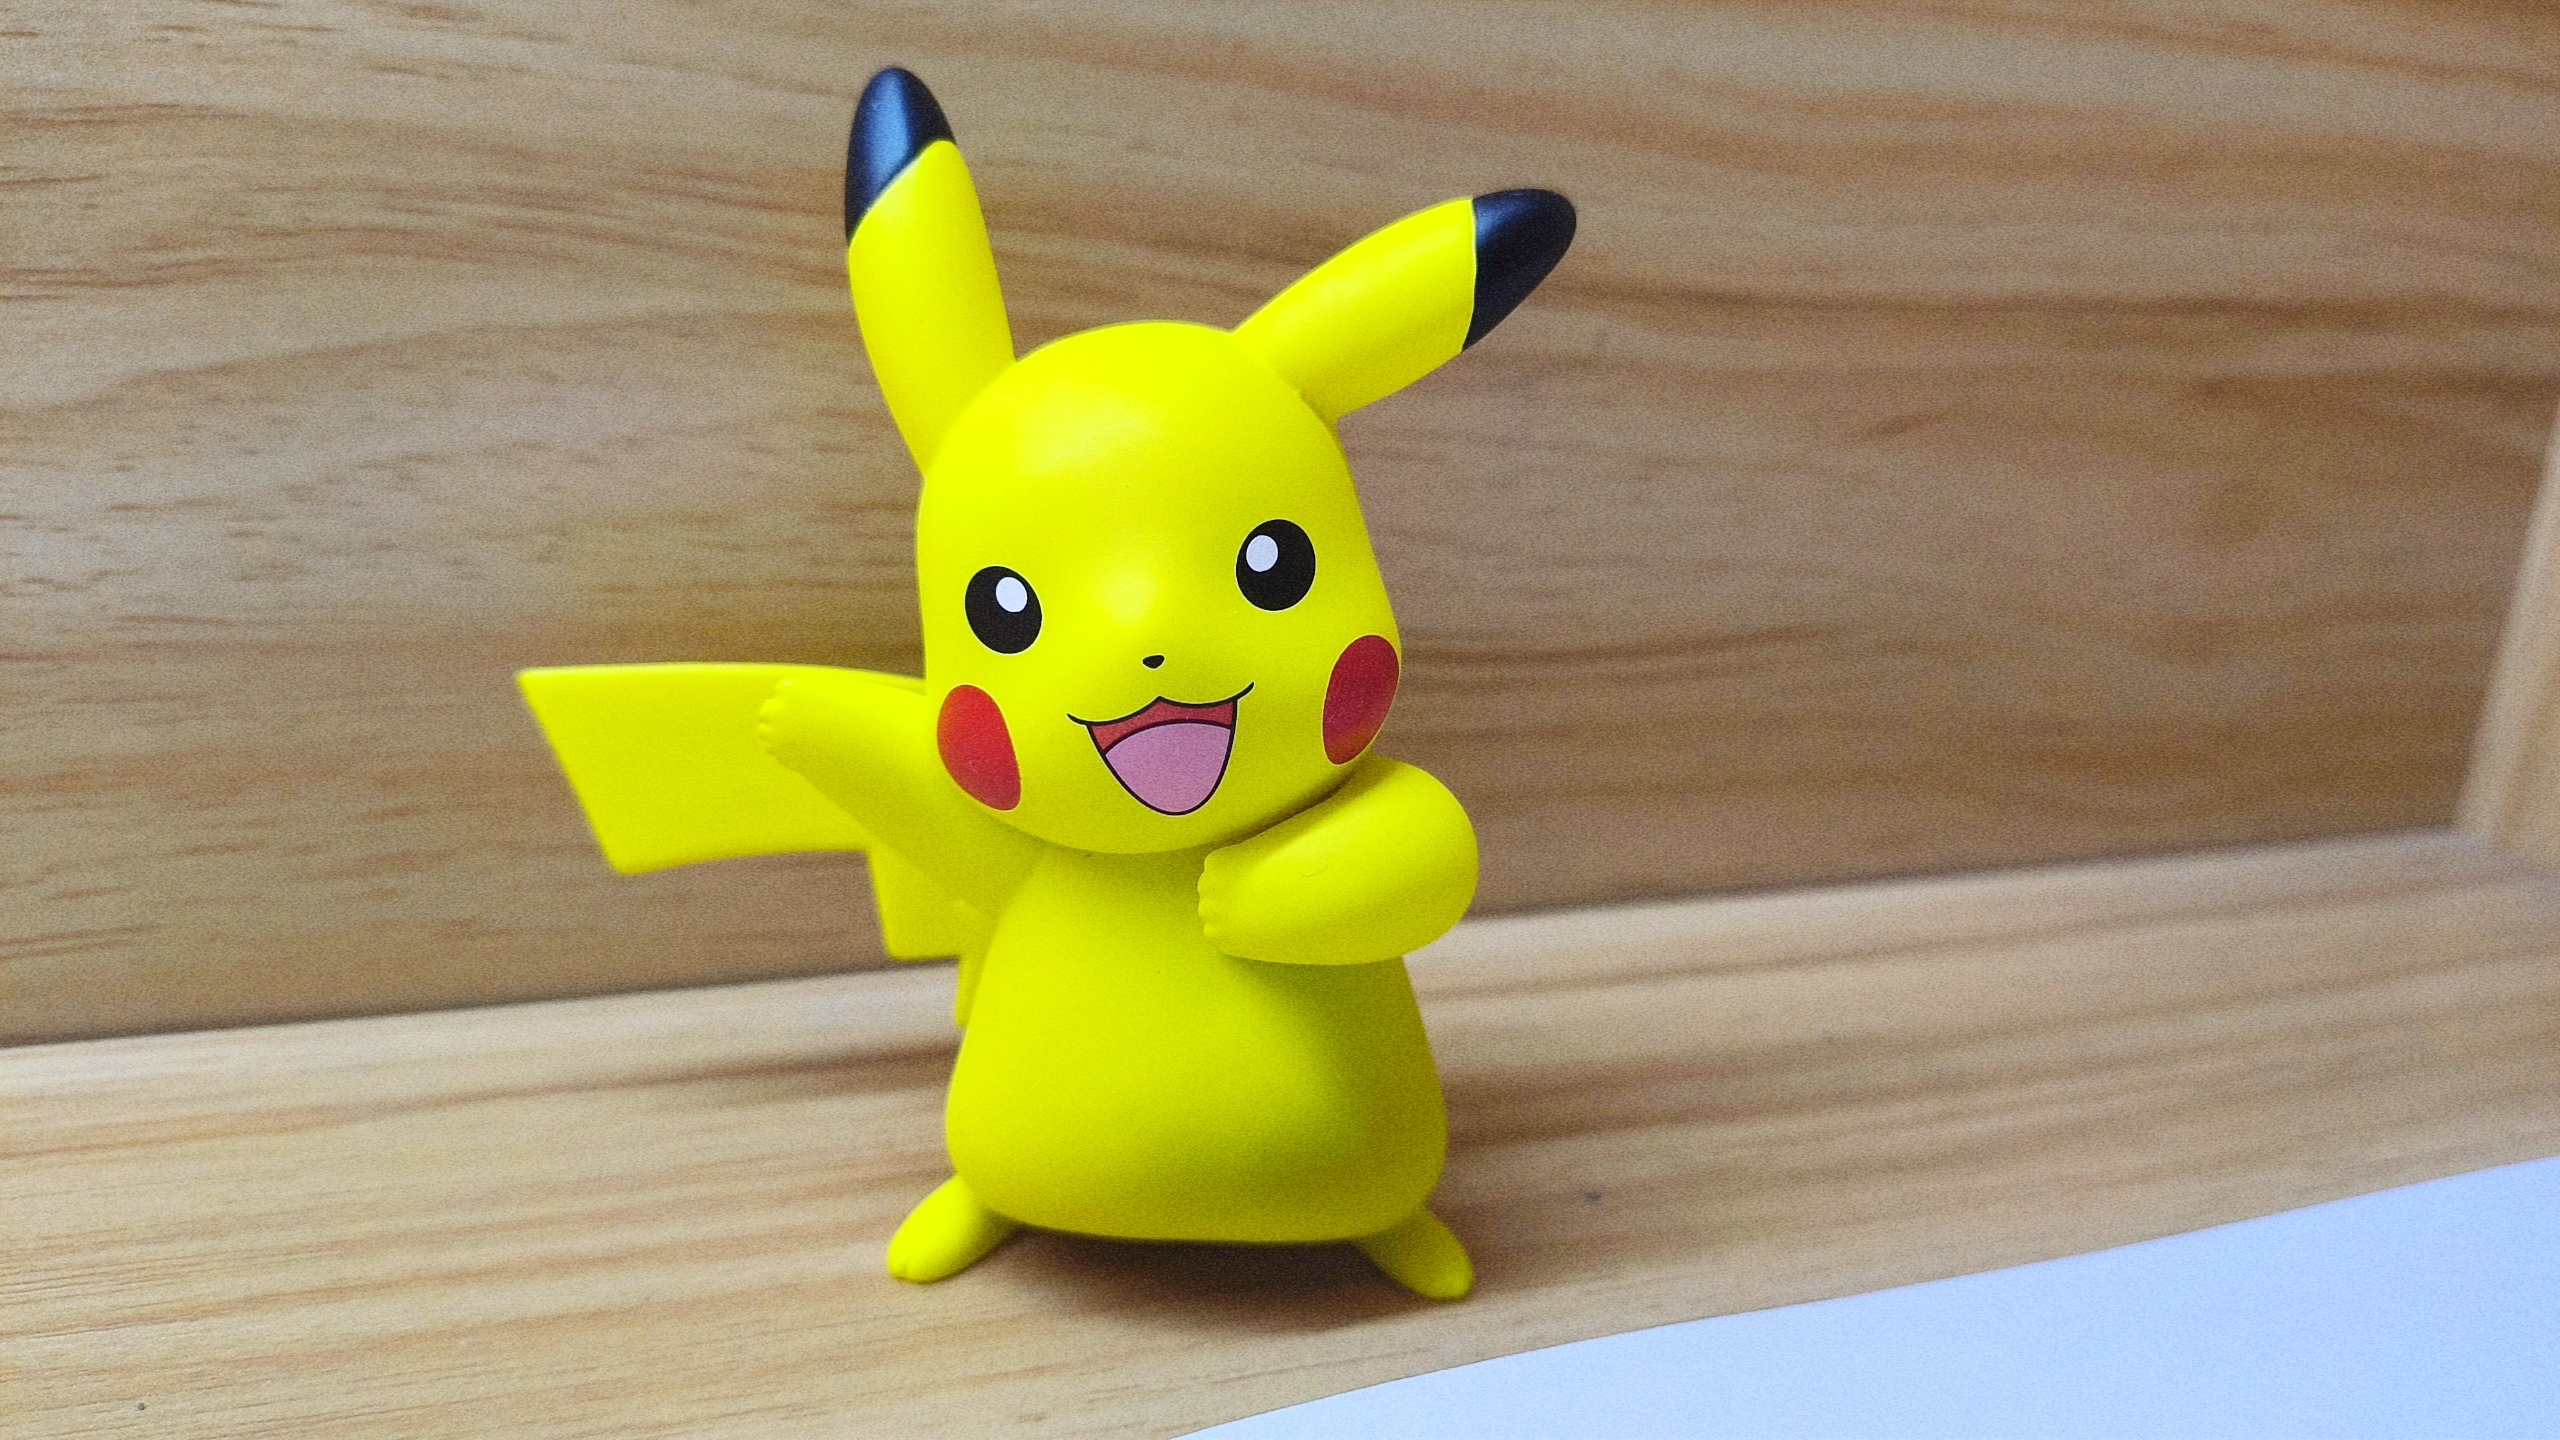
\includegraphics[scale=0.1, ]{figures/pikachu.jpg}
        \caption{这是图表}
        %\label{fig:1}
    \end{figure}

    \subsubsection{表格}

    \begin{table}[!htbp]
        \centering
        \begin{tabular}{cccccc}
            \toprule
            序号 & 姓名 & 性别 & 年龄 & 身高/cm & 体重/kg \\
            \midrule
            1 & 张三 & M & 16 & 163 & 50 \\
            2 & 王红 & F & 15 & 159 & 47 \\
            3 & 李二 & M & 17 & 165 & 52 \\
            \bottomrule
        \end{tabular}
        \caption{这是表格}
    \end{table}

    \section{基础功能测试}
    \subsection{文字与段落}
    这是文字。

    这是段落。这是段落。这是段落。这是段落。这是段落。这是段落。这是段落。这是段落。这是段落。这是段落。这是段落。这是段落。这是段落。这是段落。这是段落。这是段落。这是段落。这是段落。
    \subsubsection{文字与段落}
    这是文字。

    这是段落。这是段落。这是段落。这是段落。这是段落。这是段落。这是段落。这是段落。这是段落。这是段落。这是段落。这是段落。这是段落。这是段落。这是段落。这是段落。这是段落。这是段落。
    \subsection{图表}

    \subsubsection{图片}

    \begin{figure}[htbp]
        \centering
        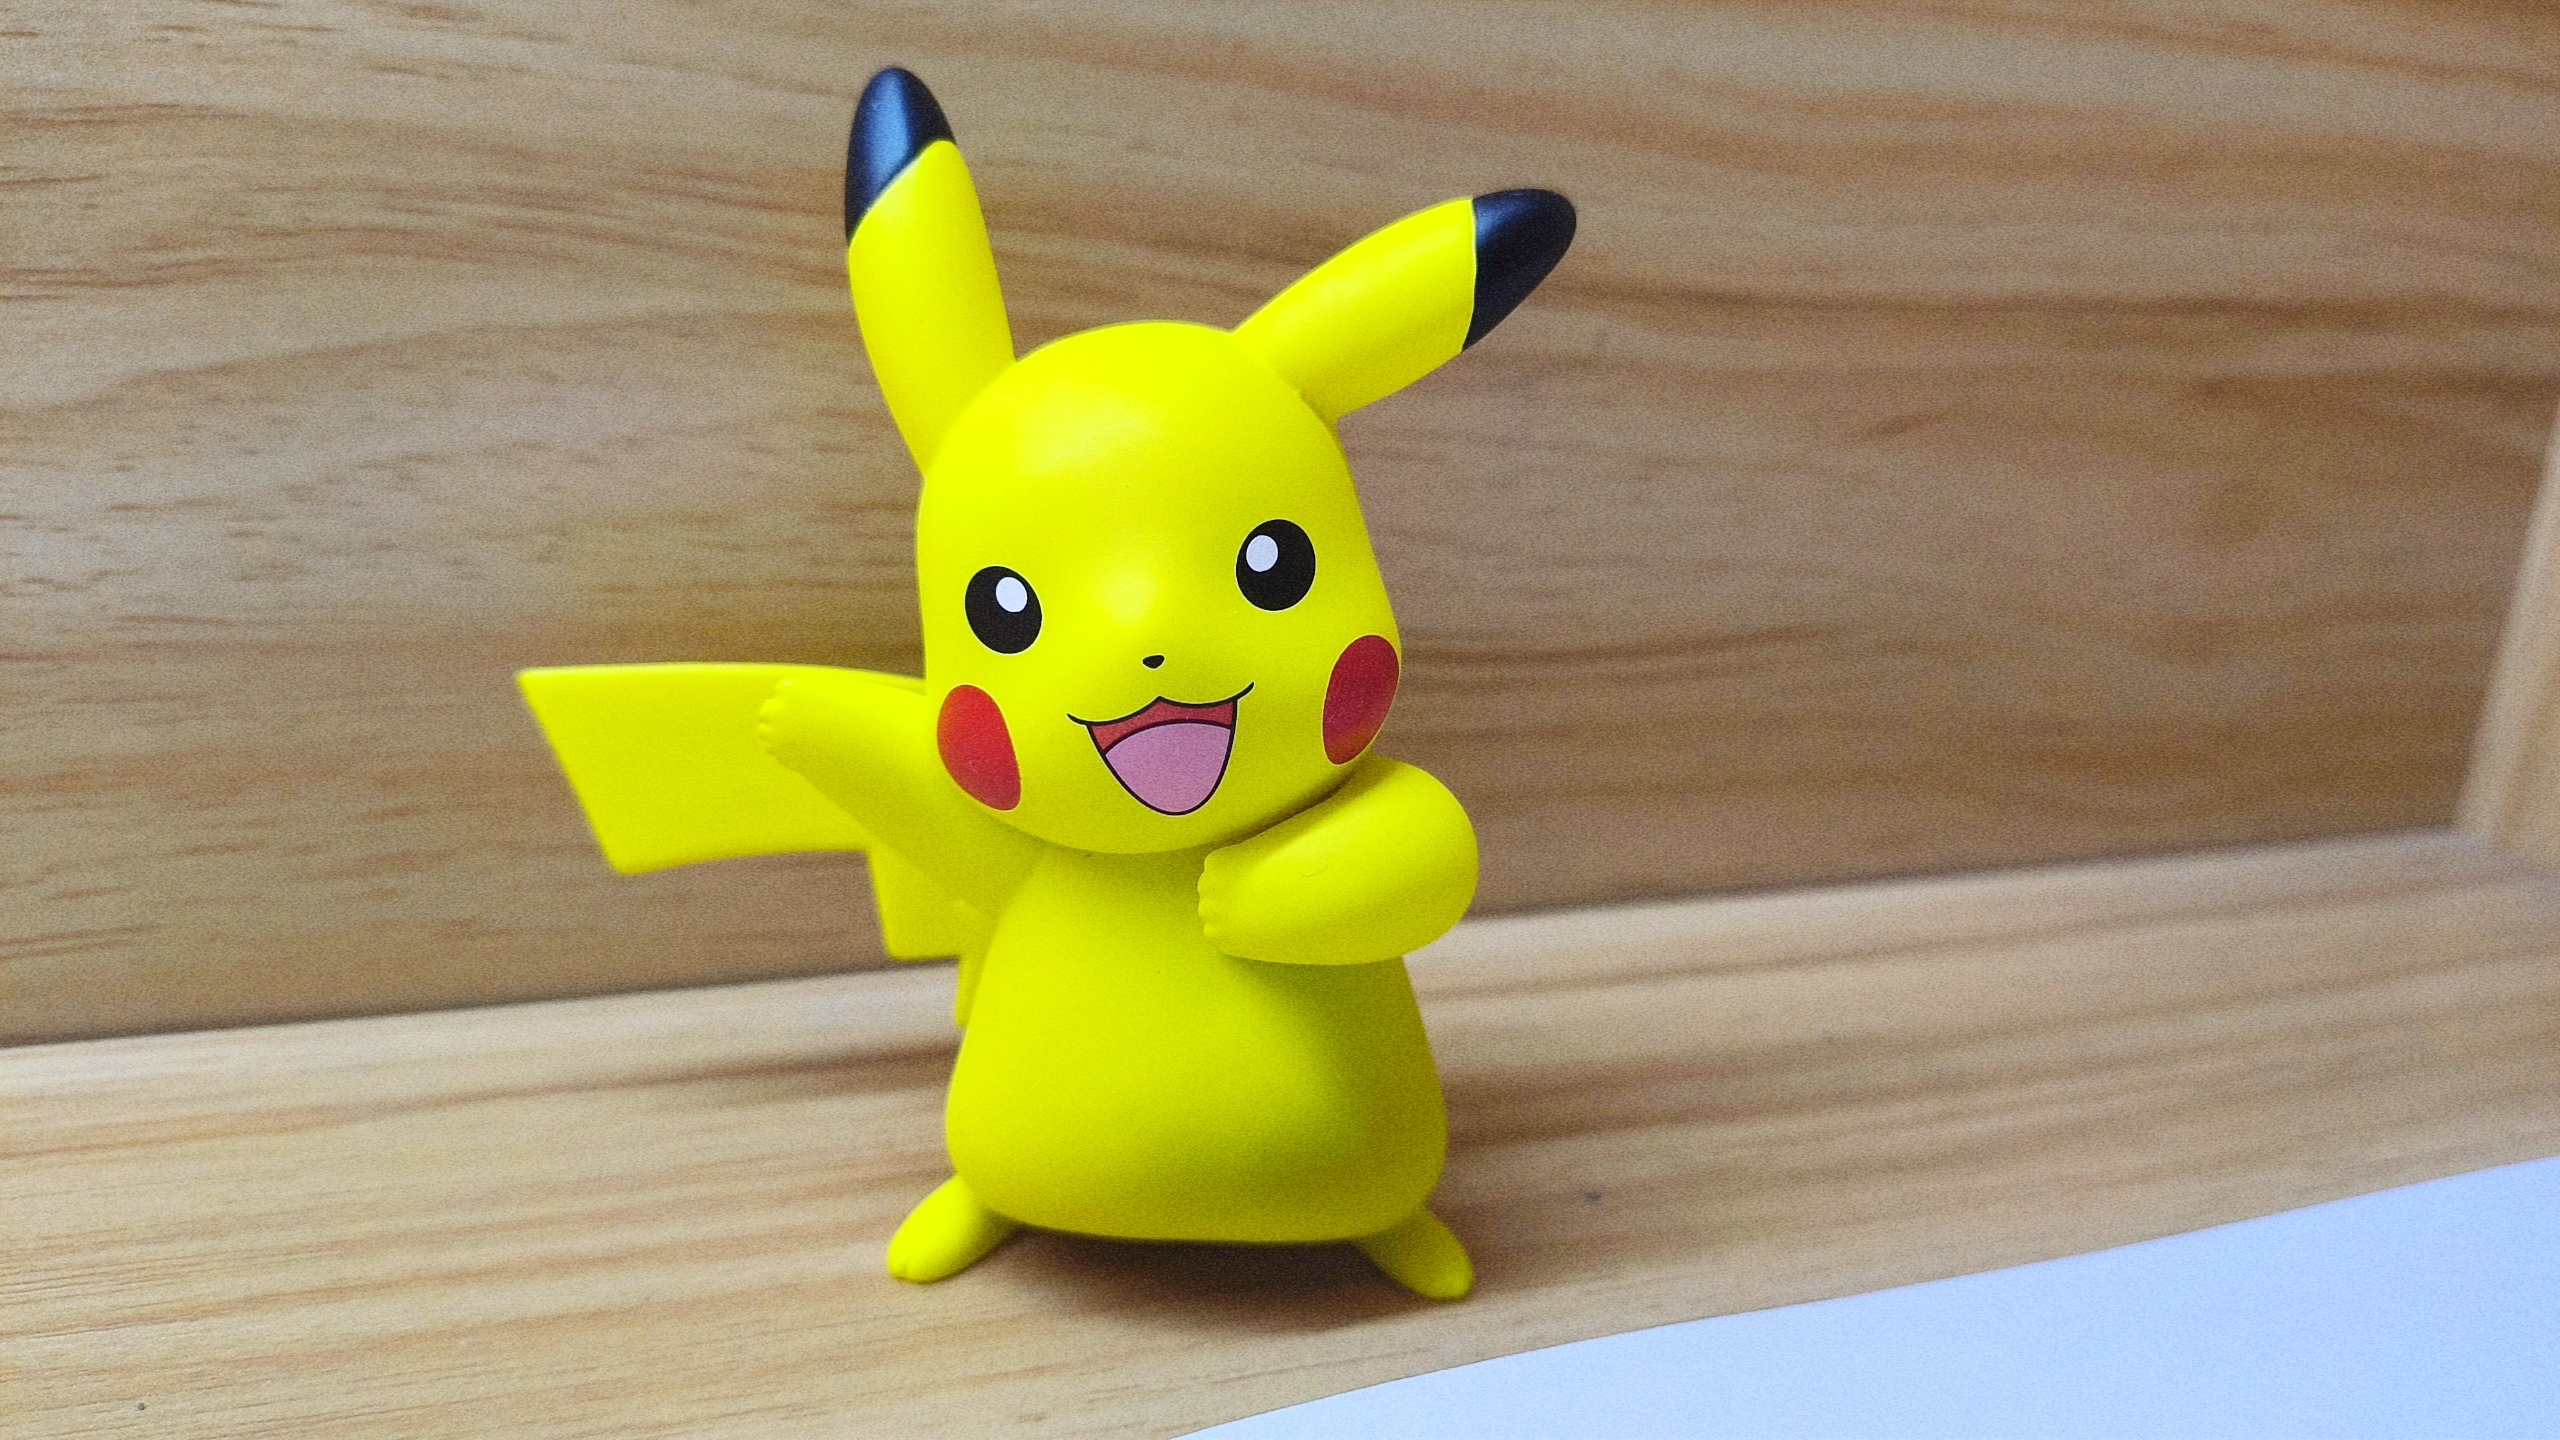
\includegraphics[scale=0.1, ]{figures/pikachu.jpg}
        \caption{这是图表}
        %\label{fig:1}
    \end{figure}

    \subsubsection{表格}

    \begin{table}[!htbp]
        \centering
        \begin{tabular}{cccccc}
            \toprule
            序号 & 姓名 & 性别 & 年龄 & 身高/cm & 体重/kg \\
            \midrule
            1 & 张三 & M & 16 & 163 & 50 \\
            2 & 王红 & F & 15 & 159 & 47 \\
            3 & 李二 & M & 17 & 165 & 52 \\
            \bottomrule
        \end{tabular}
        \caption{这是表格}
    \end{table}

    \section{基础功能测试}
    \subsection{文字与段落}
    这是文字。

    这是段落。这是段落。这是段落。这是段落。这是段落。这是段落。这是段落。这是段落。这是段落。这是段落。这是段落。这是段落。这是段落。这是段落。这是段落。这是段落。这是段落。这是段落。
    \subsubsection{文字与段落}
    这是文字。

    这是段落。这是段落。这是段落。这是段落。这是段落。这是段落。这是段落。这是段落。这是段落。这是段落。这是段落。这是段落。这是段落。这是段落。这是段落。这是段落。这是段落。这是段落。
    \subsection{图表}

    \subsubsection{图片}

    \begin{figure}[htbp]
        \centering
        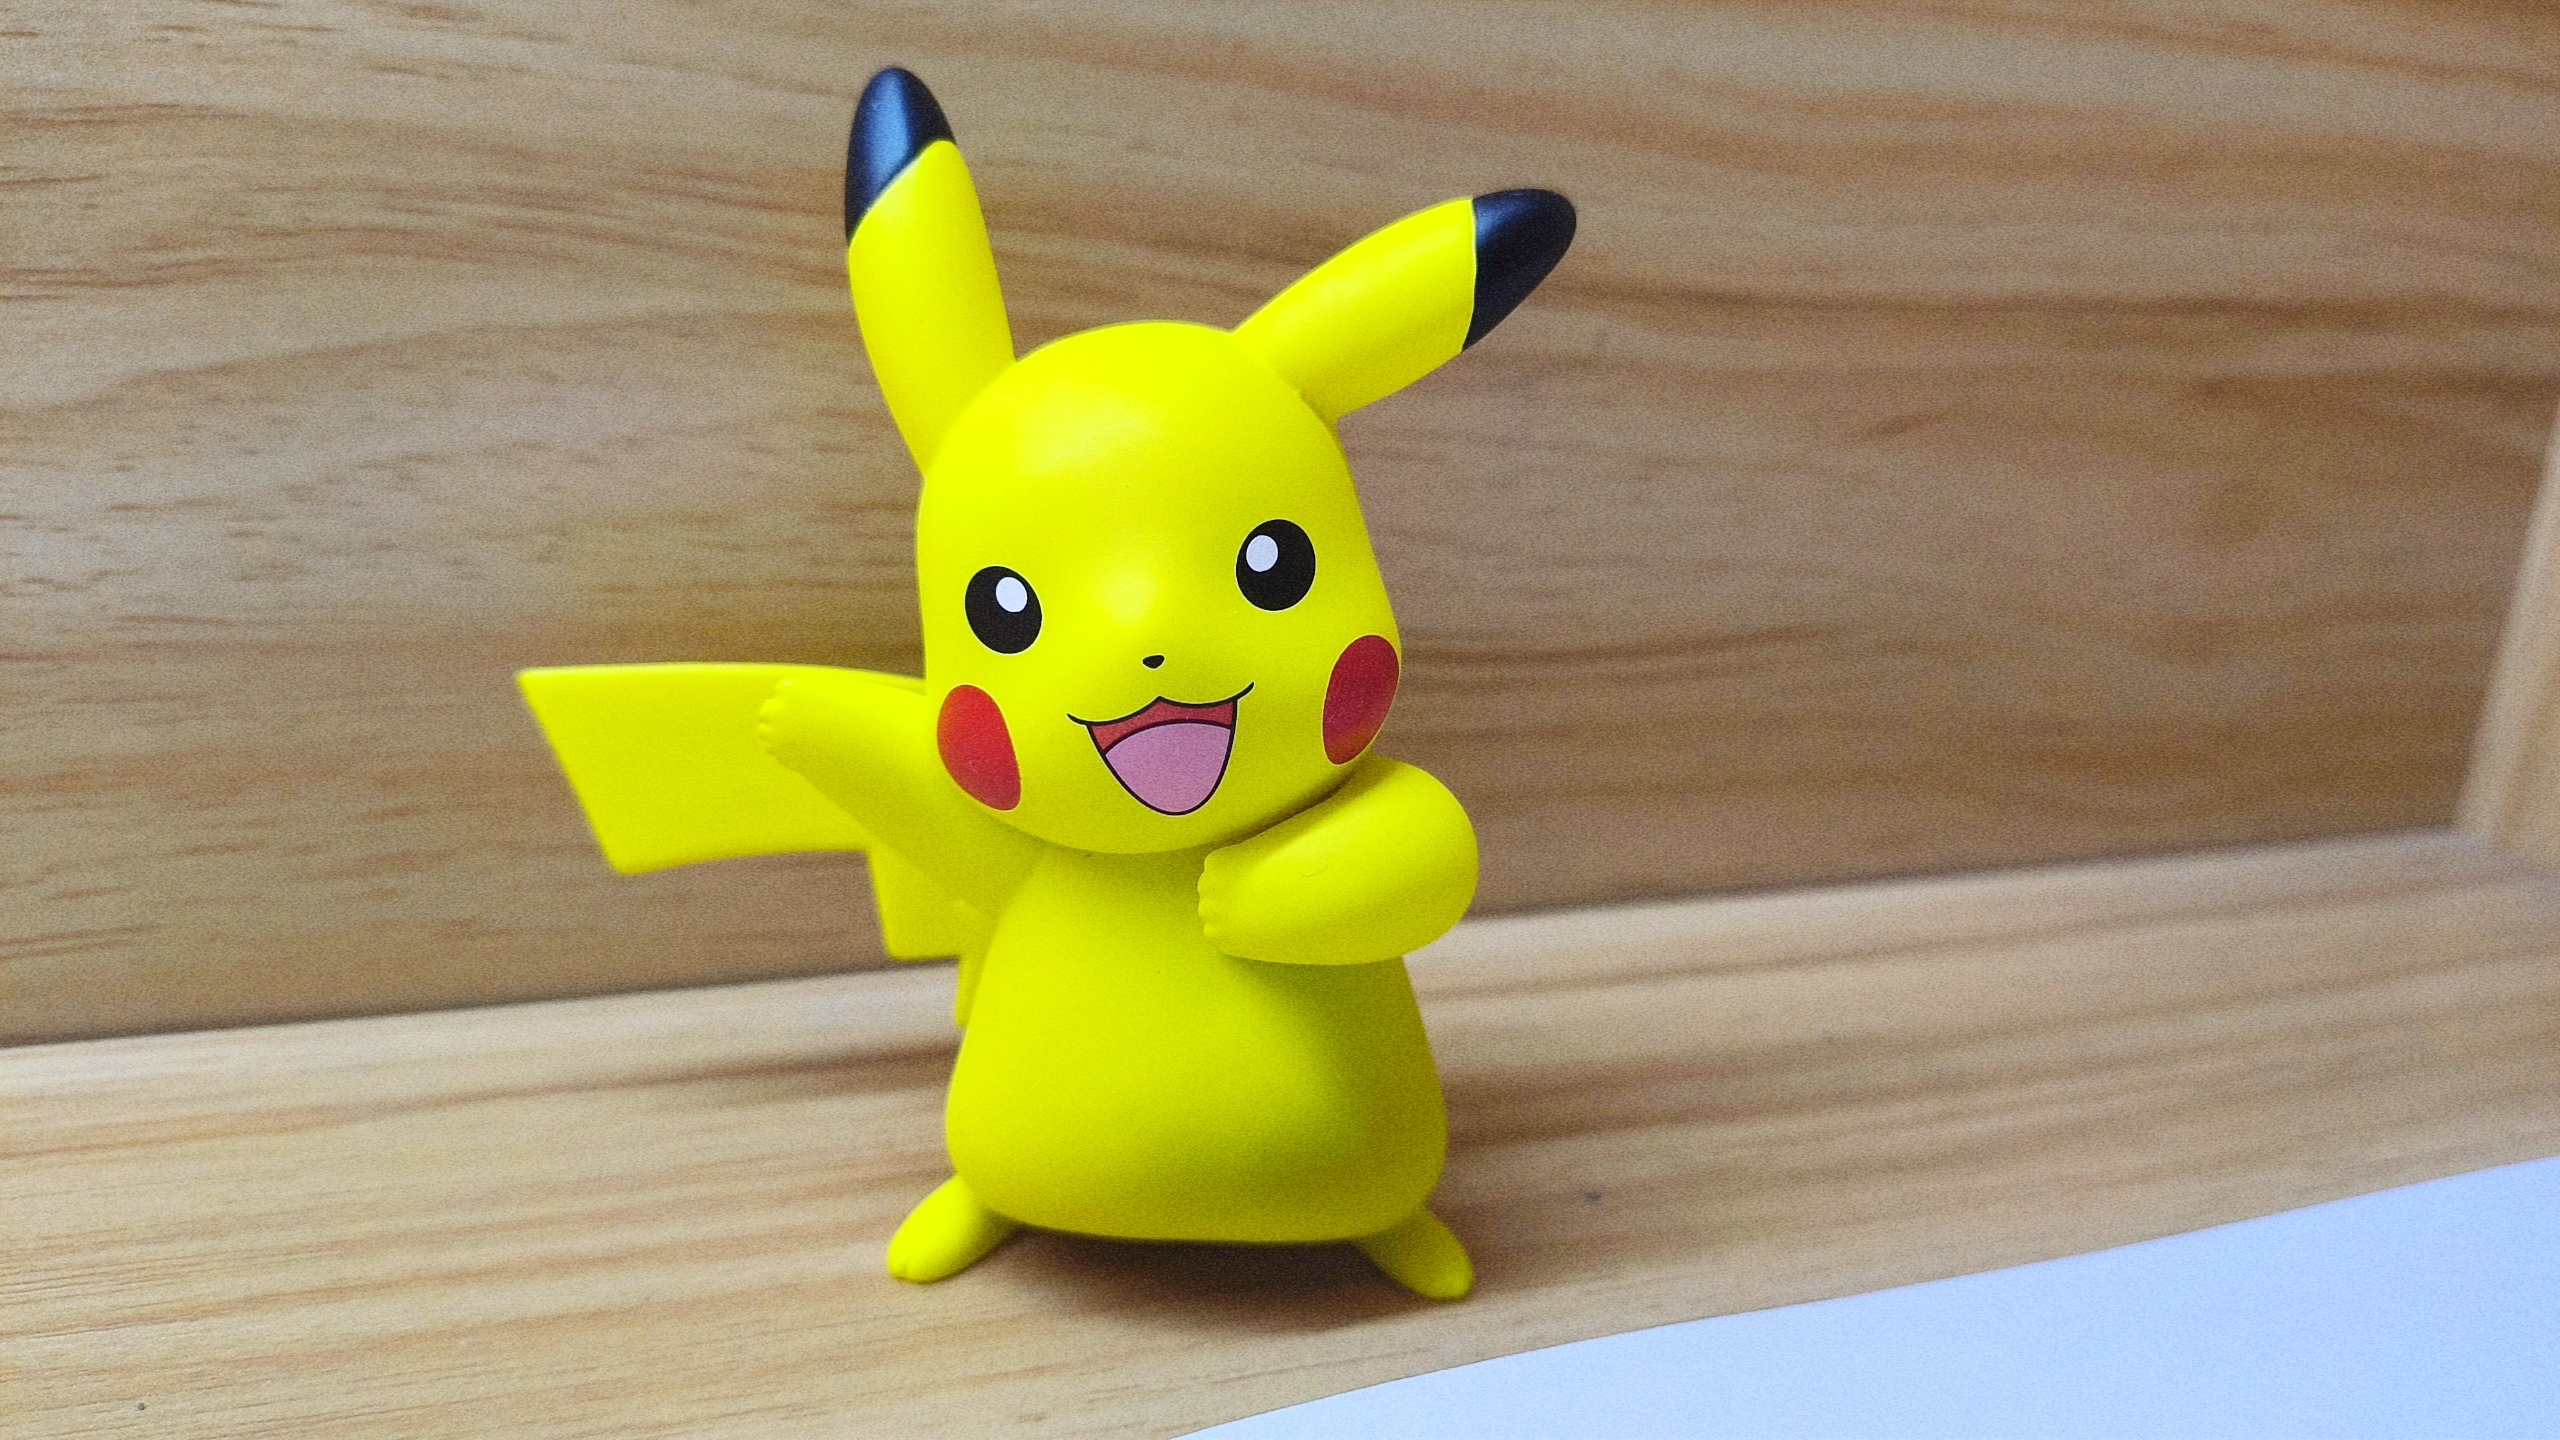
\includegraphics[scale=0.1, ]{figures/pikachu.jpg}
        \caption{这是图表}
        %\label{fig:1}
    \end{figure}

    \subsubsection{表格}

    \begin{table}[!htbp]
        \centering
        \begin{tabular}{cccccc}
            \toprule
            序号 & 姓名 & 性别 & 年龄 & 身高/cm & 体重/kg \\
            \midrule
            1 & 张三 & M & 16 & 163 & 50 \\
            2 & 王红 & F & 15 & 159 & 47 \\
            3 & 李二 & M & 17 & 165 & 52 \\
            \bottomrule
        \end{tabular}
        \caption{这是表格}
    \end{table}

\end{ujnbody}